The DAL isn't just a list as the name may suggests, it is a data structure composed of vectors and lists that are used to assist the processing of contributions of crowd workers as well as to support the generation of presentations with the synchronized videos. It was designed in order to efficiently store all relevant contributions that represent a temporal relation between a pair of videos.

Its structure is based on a Upper Triangular Matrix, although, the DAL is constructed on demand, saving space because it doesn't have any empty slot on it, turning it into a dynamic structure. In Figure~\ref{structure-dal} it is shown an instance of a DAL with five videos and its relations.

\begin{figure}[h]
	\centerline{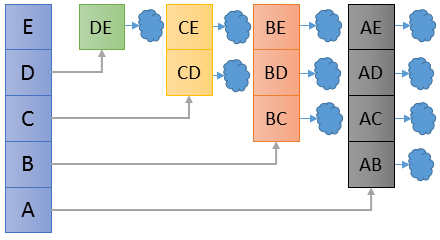
\includegraphics[scale=0.7] {figure/DAL/dal}}
	\caption{DAL Structure}
	\label{structure-dal}
\end{figure}

The DAL starts as an array that contains in its positions the videos that are going to be related (blue squares). Each video is an object that contains a reference to the media that it represents (URI) or other DAL (creating a hierarchy), a reference to the array of relations with the other videos and an attribute with the duration ($\sigma$) of the video.

These relations are cells into an array. Each position of this array is a different relation that represents the time offset between those two videos. Each position of the array stores the IDs for the pairs of videos that are being related, an attribute that contains the current $\Delta$ (time offset), an attribute that contains the degree of confidence in that relation and a list of contributions on that relation (each contribution on which is the $\Delta$ value). The degree of confidence is how precise the current $\Delta$ is believed to be true. Note that we don't need to store all direct relations (e.g. $\Delta_{A,H}$ and $\Delta_{H,A}$), we can store one direct relation and its complementary can be easily calculated ($\Delta_{A,H} = -\Delta_{H,A}$).

A contribution (in the blue cloud) in turn has the $\Delta$ proposed by each user for that relation and a reference for that user (the user profile may be used to rise the degree of confidence of a relation).